\chapter{Human-in-the-Loop (HITL): Ensuring Reliability and Control}

As LLM agents become more autonomous and are deployed in increasingly critical business functions, ensuring their reliability, safety,
 and alignment with human expectations is paramount. Human-in-the-Loop (HITL) is an essential design philosophy and set of practices
  that integrate human judgment and oversight into agentic systems. It is not a sign of automation failure, but rather a strategic 
  approach to building more robust, trustworthy, and effective AI solutions.

\section{The Importance of HITL in Agentic Systems}
The integration of HITL is crucial for several reasons, primarily stemming from the inherent limitations of current LLM technology 
and the need for accountability in automated decision-making:
\begin{itemize}
    \item \textbf{Addressing LLM Limitations:} Despite their advancements, LLMs can still "hallucinate" (generate plausible but incorrect information), 
    exhibit biases present in their training data, or lack true understanding of complex nuances. HITL provides a mechanism to catch and correct 
    these errors before they lead to negative consequences.
    \item \textbf{Ensuring Safety and Reliability:} For tasks that are critical or sensitive—such as financial transactions, medical advice or 
    actions, legal document generation, or modifications to production systems—allowing fully autonomous agent operation without human verification 
    can be risky. HITL allows human experts to validate an agent's proposed actions or outputs, especially when stakes are high. 
    For example, user confirmation is a straightforward way to pause and validate specific actions before execution.
    \item \textbf{Building User Trust and Managing Accountability:} When users know that a human can review or intervene in an 
    AI agent's process, it can significantly increase their trust in the system. Furthermore, HITL helps clarify accountability; 
    if an error occurs, the points of human oversight are identifiable.
    \item \textbf{Handling Edge Cases and Ambiguity:} AI agents may encounter novel situations, ambiguous queries, or scenarios
     where their confidence in a particular decision is low. HITL allows the agent to escalate these situations to a 
     human who can apply domain expertise, common sense, or contextual understanding that the agent may lack.
    \item \textbf{Facilitating Continuous Improvement:} Human feedback is invaluable for the ongoing improvement of LLM agents.
     When humans correct errors, refine outputs, or label data where the agent struggled, this information can be used to 
     fine-tune the underlying LLM, improve prompt engineering, or enhance tool design, leading to better performance over time. 
     This is a core principle of Reinforcement Learning from Human Feedback (RLHF).
    \item \textbf{Ethical Oversight:} HITL allows for the incorporation of ethical considerations and human values into the agent's operation, 
    helping to mitigate bias and ensure fair outcomes.
\end{itemize}
For software engineers, designing for HITL means architecting systems with explicit checkpoints for human review, intervention, and override. 
This is a strategic design choice that acknowledges the current capabilities and limitations of AI, leveraging human strengths—such as judgment, 
nuanced contextual understanding, and ethical reasoning—to complement the AI's speed and data processing capabilities. 
This collaborative approach leads to more dependable and trustworthy AI solutions, which is particularly important as agents are 
given more responsibility in enterprise settings.

\section{Common HITL Workflow Patterns}
There are several common patterns for integrating Human-in-the-Loop into LLM agent workflows, each suited to different needs and stages of the agent's operation:

\subsection*{Review and Approval}
This is one of the most common HITL patterns, especially for actions that have significant consequences or are irreversible.
\begin{itemize}
    \item \textbf{Workflow:} The LLM agent processes a request, determines a course of action (e.g., sending an email, updating a 
    database record, executing a financial transaction), or generates content (e.g., a legal clause, a customer response). 
    Before the action is executed or the content is finalized, it is presented to a human reviewer. 
    The human can then approve the action/content, reject it, or edit it.
    \item \textbf{Example:} An agent drafts a response to a critical customer complaint. A human support manager reviews and 
    approves (or modifies) the draft before it's sent to the customer. Amazon Bedrock Agents, for instance, offer an 
    out-of-the-box user confirmation feature for this purpose.
\end{itemize}

\subsection*{Data Labeling/Annotation for Continuous Improvement (RLHF)}
This pattern focuses on improving the agent's underlying LLM or its training data over time.
\begin{itemize}
    \item \textbf{Workflow:} When the agent encounters data it's uncertain about (e.g., an ambiguous user query, a difficult-to-classify image),
     or as part of a regular quality control process, these data points are sent to human annotators. Humans provide correct labels,
      rank responses, or offer corrections. This curated feedback is then used to fine-tune the LLM or improve the knowledge base it uses.
    \item \textbf{Example:} An LLM agent used for sentiment analysis flags customer reviews where its confidence in the sentiment
     classification is low. Human reviewers then label these ambiguous reviews, and this new labeled data is used to retrain or
      fine-tune the sentiment analysis model.
\end{itemize}

\subsection*{Exception Handling and Escalation}
This pattern is used when the agent is unable to complete a task, encounters an error it cannot resolve, or its confidence in a
 decision falls below a predefined threshold.
\begin{itemize}
    \item \textbf{Workflow:} The agent attempts to perform its task. If it fails or determines it cannot proceed reliably, 
    it "escalates" the task, along with all relevant context, to a human operator or expert.
    \item \textbf{Example:} A customer service chatbot tries to resolve a technical issue using its available tools and knowledge. 
    If it exhausts its options or the customer indicates the problem is still not solved, the chatbot transfers the conversation 
    (including the history) to a human support agent. The \texttt{KnowNo} framework, for example, triggers human queries when
     the LLM's confidence in a plan is low.
\end{itemize}

\subsection*{Interactive Refinement (Collaborative Generation)}
In this pattern, the human user and the LLM agent work together iteratively to produce a desired output.
\begin{itemize}
    \item \textbf{Workflow:} The agent generates an initial draft or proposes a solution. The human user reviews it and provides
     feedback, suggestions, or corrections. The agent then revises its output based on this feedback. This cycle can repeat multiple 
     times until the user is satisfied.
    \item \textbf{Example:} A software developer uses an LLM agent to generate a piece of code. The developer reviews the generated code, 
    points out areas for improvement or bugs, and asks the agent to refine it. The agent incorporates the feedback and produces an updated
     version of the code. Frameworks like \texttt{LangGraph} support "interrupt" functionalities to pause agent execution and await user
      input for such scenarios.
\end{itemize}

The following table summarizes these common HITL workflow patterns, providing a quick reference for engineers.
% For a proper table spanning text width and with better line wrapping, consider using packages like 'tabularx' or 'tabulary'.
% The following is a basic implementation.
\begin{table}[h!]
\centering
\caption{HITL Workflow Patterns Overview}
\label{tab:hitl_patterns}
\begin{tabular}{|p{0.2\linewidth}|p{0.25\linewidth}|p{0.25\linewidth}|p{0.25\linewidth}|}
\hline
\textbf{Pattern Name} & \textbf{Description} & \textbf{When to Use} & \textbf{Example Scenario} \\
\hline
Review \& Approval & Agent proposes action/content; human validates before execution/release. & Critical actions, irreversible operations, 
high-stakes content generation. & Agent proposes a financial transaction; human accountant approves before execution. \\
\hline
Data Annotation for RLHF & Humans label data where the model is uncertain or for quality control, feeding back into model training. & Improving model
 accuracy over time, handling ambiguous data, specializing models for new domains. & Agent flags unclear customer queries; humans categorize them
  to improve future intent recognition. \\
\hline
Exception Handling \& Escalation & Agent escalates to a human when it fails, confidence is low, or a predefined error condition is met. & Unforeseen situations, 
tasks requiring expertise beyond agent's capability, ensuring task completion. & Automated IT support agent cannot resolve a network issue 
and escalates to a human network engineer with logs. \\
\hline
Interactive Refinement & Human and agent collaborate iteratively to create or refine an output. & Creative tasks (writing, coding), 
complex problem-solving where human guidance is beneficial throughout. & Agent generates a marketing slogan; human marketer provides 
feedback for tone and style; agent revises. \\
\hline
\end{tabular}
\end{table}

Choosing the right HITL pattern, or a combination of patterns, depends on the specific application, the level of risk involved, 
the need for accuracy, and the desired degree of user control. These patterns are not mutually exclusive and can often be combined 
within a single agentic application to create a robust and reliable system.

\section{Implementing HITL in Your Agentic Applications (with Block Diagram)}
Successfully implementing Human-in-the-Loop workflows in agentic applications requires careful architectural considerations to 
ensure seamless collaboration between the LLM agent and human reviewers or operators.

\subsection*{Architectural Considerations}
\begin{itemize}
    \item \textbf{Explicit Pause/Interrupt Points:} The agent's workflow must be designed with clearly defined points where 
    execution can be paused to await human input or approval. This often involves using specific mechanisms provided by agent
     frameworks (like \texttt{LangGraph}'s \texttt{interrupt()} function) or custom logic.
    \item \textbf{State Persistence:} When an agent pauses, its current state—including the task context, conversation history,
     any intermediate results, and the proposed action or data needing review—must be reliably persisted. This is crucial because human 
     review might not be instantaneous; it could take minutes, hours, or even days. Durable Objects or similar database solutions can be used for this.
    \item \textbf{Human Review Interface (UI/UX):} A well-designed user interface is needed for human reviewers. This interface should clearly present:
    \begin{itemize}
        \item The context of the task.
        \item The agent's proposed action or the data requiring review.
        \item Any relevant supporting information or the agent's reasoning (if available).
        \item Clear options for the human to approve, reject, edit, or provide feedback.
    \end{itemize}
    \item \textbf{Resumption Logic:} Once human input is provided, the system must be able to resume the agent's workflow, incorporating 
    the human's decision or feedback into the agent's state.
    \item \textbf{Logging and Auditing:} All HITL interactions, including what was presented to the human, the human's input, and the timestamp, 
    should be logged for auditing, traceability, and potential analysis for system improvement.
    \item \textbf{Error Handling and Timeouts:} The system should gracefully handle scenarios like reviewer unavailability or timeouts for review, 
    potentially with escalation paths or default actions.
\end{itemize}

\subsection*{Generic Block Diagram for an HITL System in an LLM Agent}
The following diagram illustrates a conceptual workflow for an LLM agent incorporating a Human-in-the-Loop checkpoint:

\begin{figure}[htbp]
    \centering
    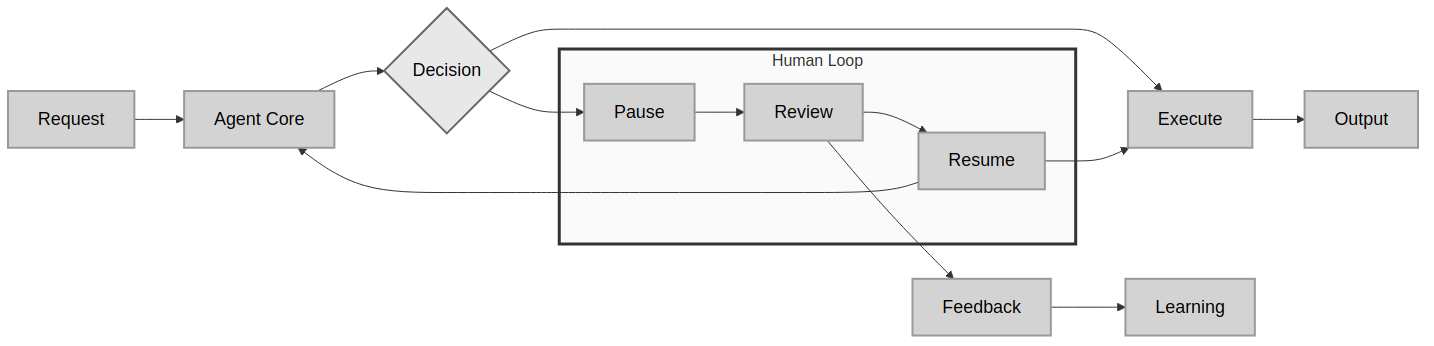
\includegraphics[width=\textwidth]{diagrams/hitl_system.png}
    \caption{Block Diagram of an HITL System in an LLM Agent}
    \label{fig:hitl_system}
\end{figure}

\subsection*{Explanation of Diagram}
\begin{itemize}
    \item \textbf{User Request:} The process starts with a request or goal provided to the LLM Agent Core.
    \item \textbf{Agent Processing:} The agent engages in its typical cycle of planning, reasoning, and tool use.
    \item \textbf{Decision Point / Confidence Check:} At certain pre-defined points in its workflow, or when its confidence in a decision or 
    action is below a threshold, the agent reaches a Decision Point.
    \item \textbf{Autonomous Path:} If confidence is high and the risk is low (or no HITL trigger is met), the agent proceeds to 
    Execute Action / Finalize Output and then provides the output to the user.
    \item \textbf{HITL Path:} If confidence is low, risk is high, or a specific HITL trigger is activated, the agent's current operation is Paused, 
    and its State is Persisted.
    \item \textbf{Human Review Interface:} The relevant information (context, proposed action, agent's reasoning if available) is 
    presented to a human reviewer through a dedicated Human Review Interface.
    \item \textbf{Human Input:} The human reviewer provides input (e.g., approves, edits, rejects the proposed action, or provides 
    clarifying feedback).
    \item \textbf{Resume Agent Logic:} The agent's workflow is resumed. Based on the human's input:
    \begin{itemize}
        \item If approved or edited, the agent may proceed to Execute Action / Finalize Output.
        \item If rejected or if significant re-planning is needed, the agent might loop back to its LLM Agent Core to reconsider its plan 
        with the new human feedback.
    \end{itemize}
    \item \textbf{Feedback Collection:} The human's feedback can also be systematically collected and stored.
    \item \textbf{Agent Learning \& Fine-tuning:} This collected feedback can be used in an offline process to fine-tune the LLM, improve prompts, 
    or refine tool usage, leading to continuous improvement of the agent.
\end{itemize}
Implementing HITL effectively is more than just adding a conditional check for human review. It requires thoughtful design of the agent's 
state management, task queuing mechanisms (if reviews are asynchronous), and user interfaces to ensure a productive and seamless collaboration 
between human intelligence and AI capabilities. This approach is fundamental to building agentic systems that are not only powerful but also 
safe, reliable, and aligned with enterprise requirements.
